\clearpage
\newpage


\section{Segmentação Semântica Baseada em Aprendizado Profundo}
\label{semantic}
No contexto das segmentações baseadas em técnicas de \textit{deep learning} com uma vertente mais específica das CNNs, a segmentação semântica se destaca por atribuir uma classe ou rótulo específico a cada pixel em uma cena \citep{Wang2017, Ghosh2019, Shelhamer2016, Arbelaez2012, Zhang2018}, constituindo, assim, um trabalho em nível de pixel.

O emprego de técnicas de segmentação semântica tem demonstrado utilidade em cenários onde o contexto é desconhecido, permitindo compreender a categoria dos objetos presentes na cena, além de suas propriedades de localização, espacialidade, dimensionalidade e formatos \citep{Zhang2018}. Essas abordagens são de extrema importância em áreas como imagens médicas, sistemas autônomos e campos correlatos.

Normalmente, as saídas das redes de segmentação semântica consistem em máscaras de \textit{pixels} organizadas como mapas de características, mapeando todas as classes na imagem original. Um exemplo visual dessa saída pode ser observado especificamente na Figura \ref{semantic:fig:3.2}, tendo a Figura \ref{semantic:fig:3.1} como referência da imagem original.

\begin{figure}[H]
   \caption{Segmentação semântica.}
   \centering
   \label{semantic:fig:3}
    \begin{subfigure}[t]{0.45\textwidth}
        \centering
        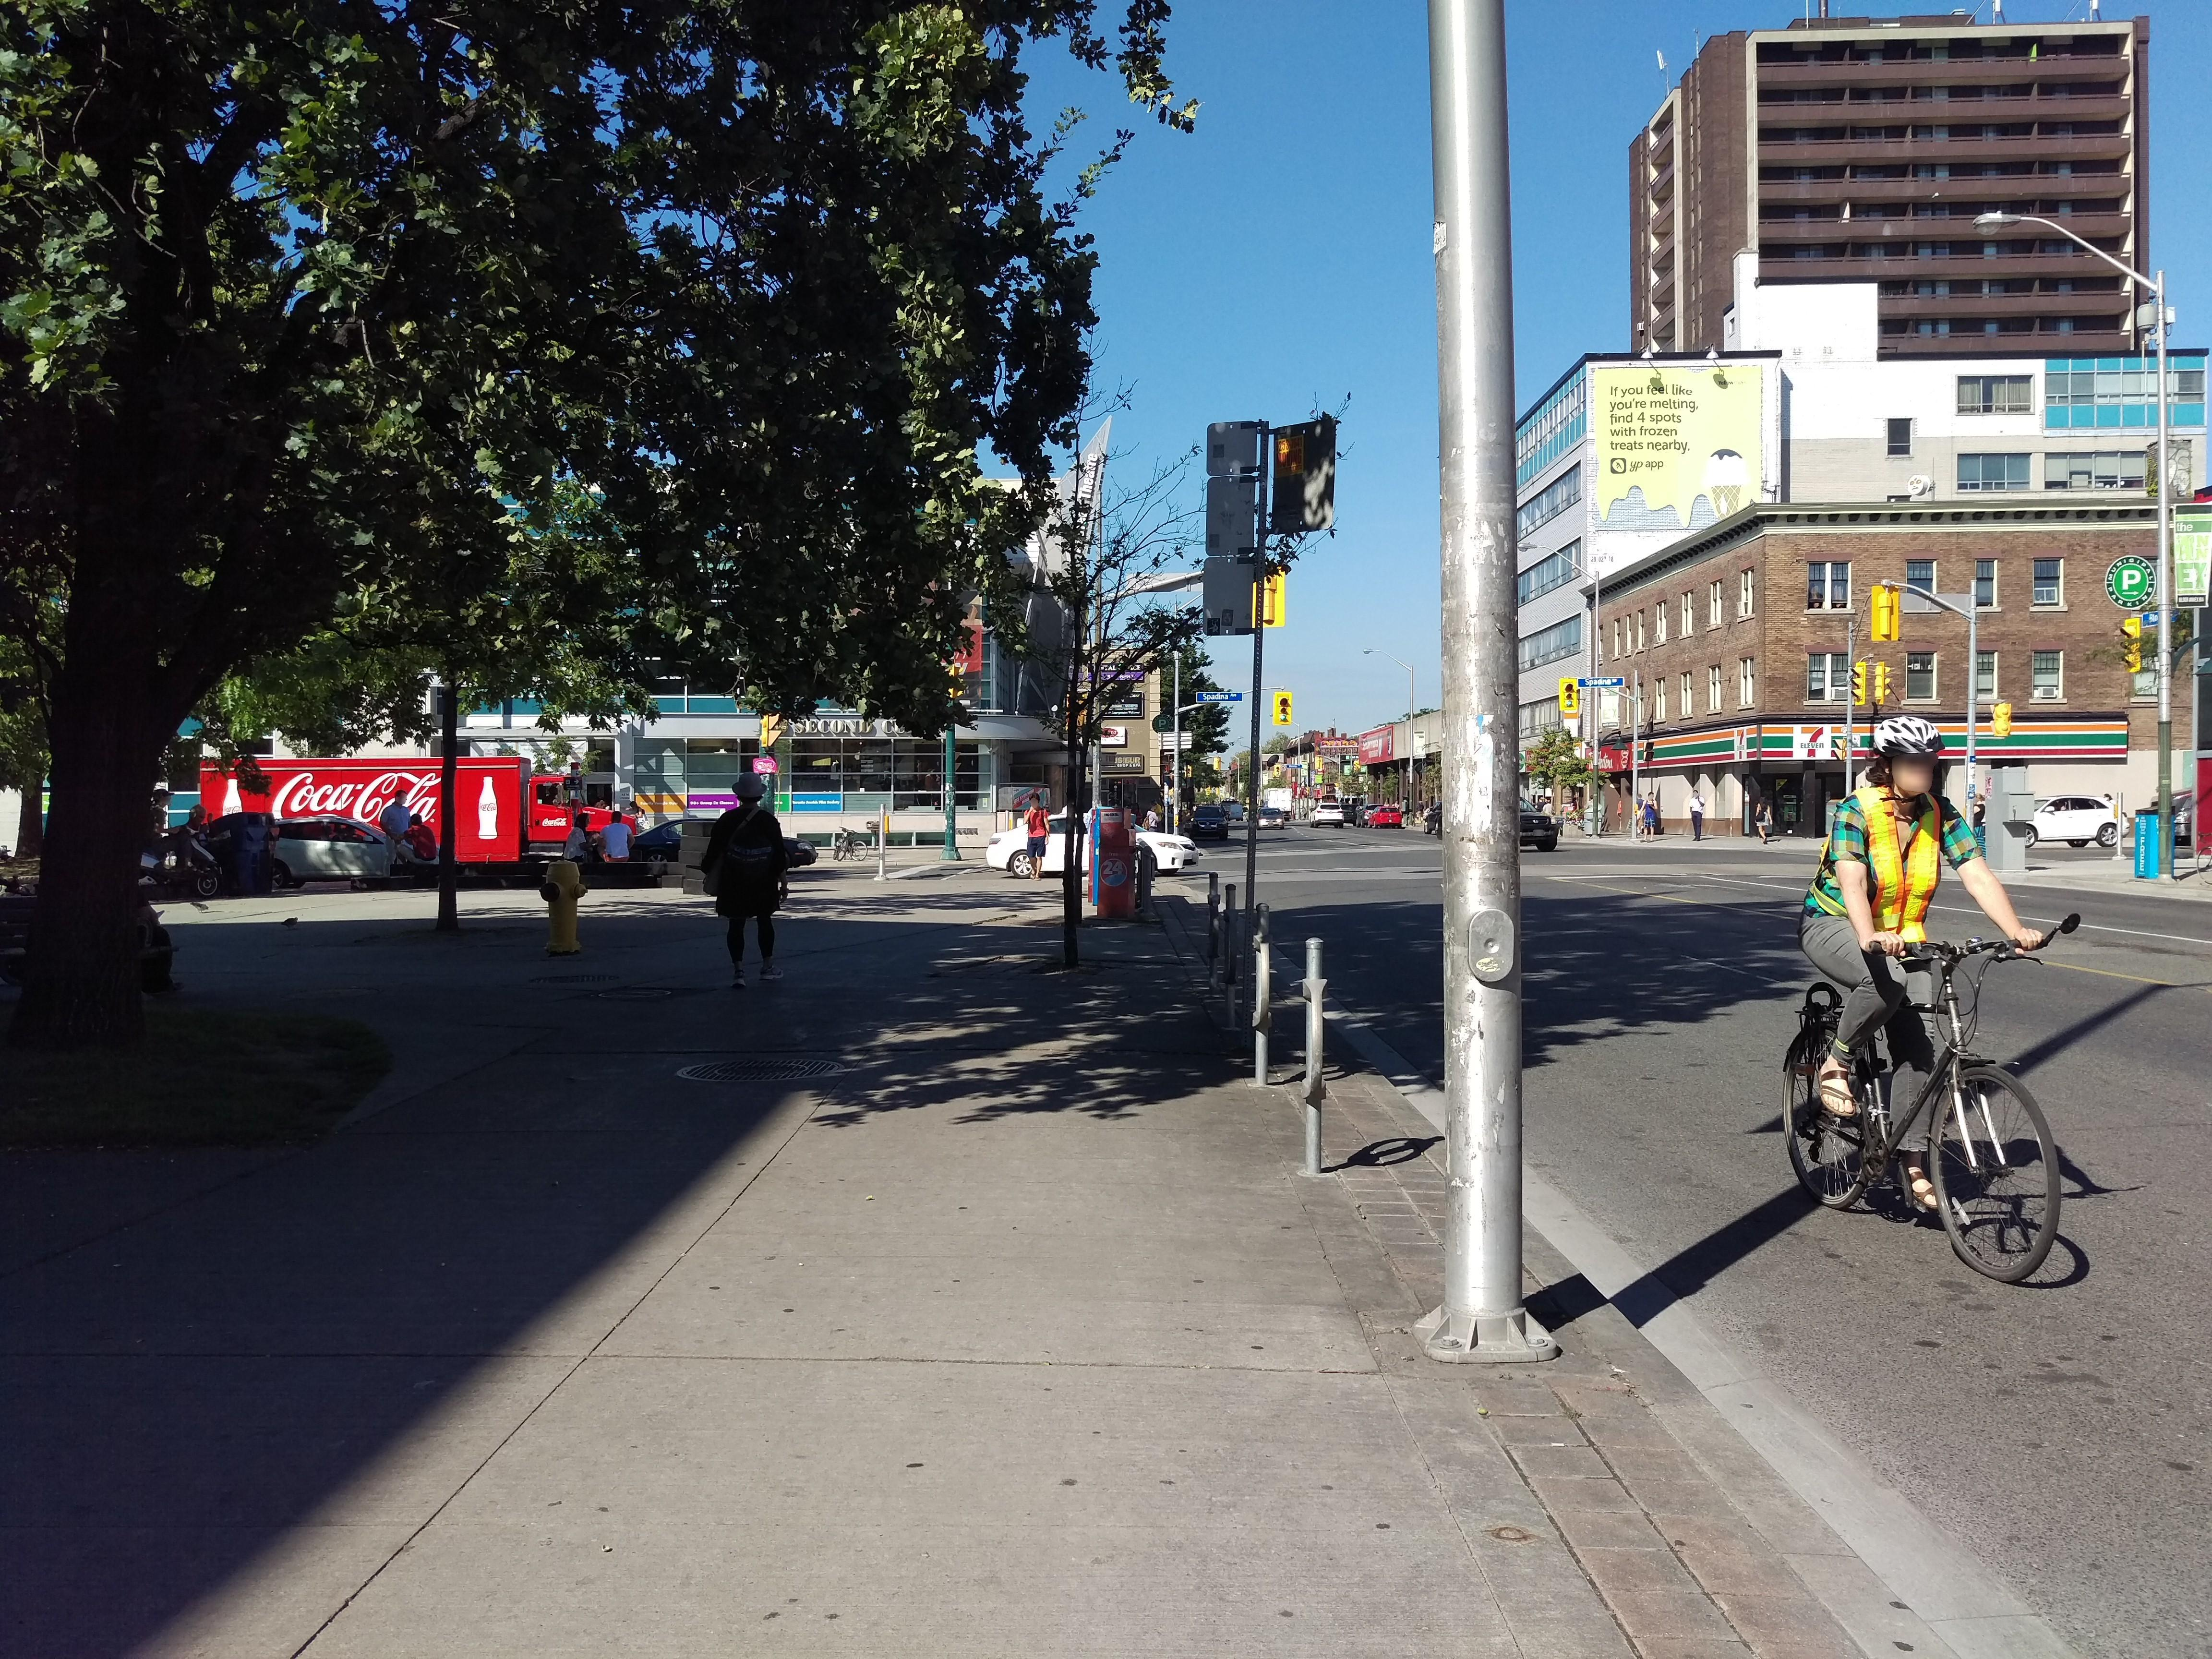
\includegraphics[height=1.5in]{recursos/imagens/semantic/t1.jpg}
        \caption{Imagem original.}
        \label{semantic:fig:3.1}
    \end{subfigure}%
    ~ 
    \begin{subfigure}[t]{0.45\textwidth}
        \centering
        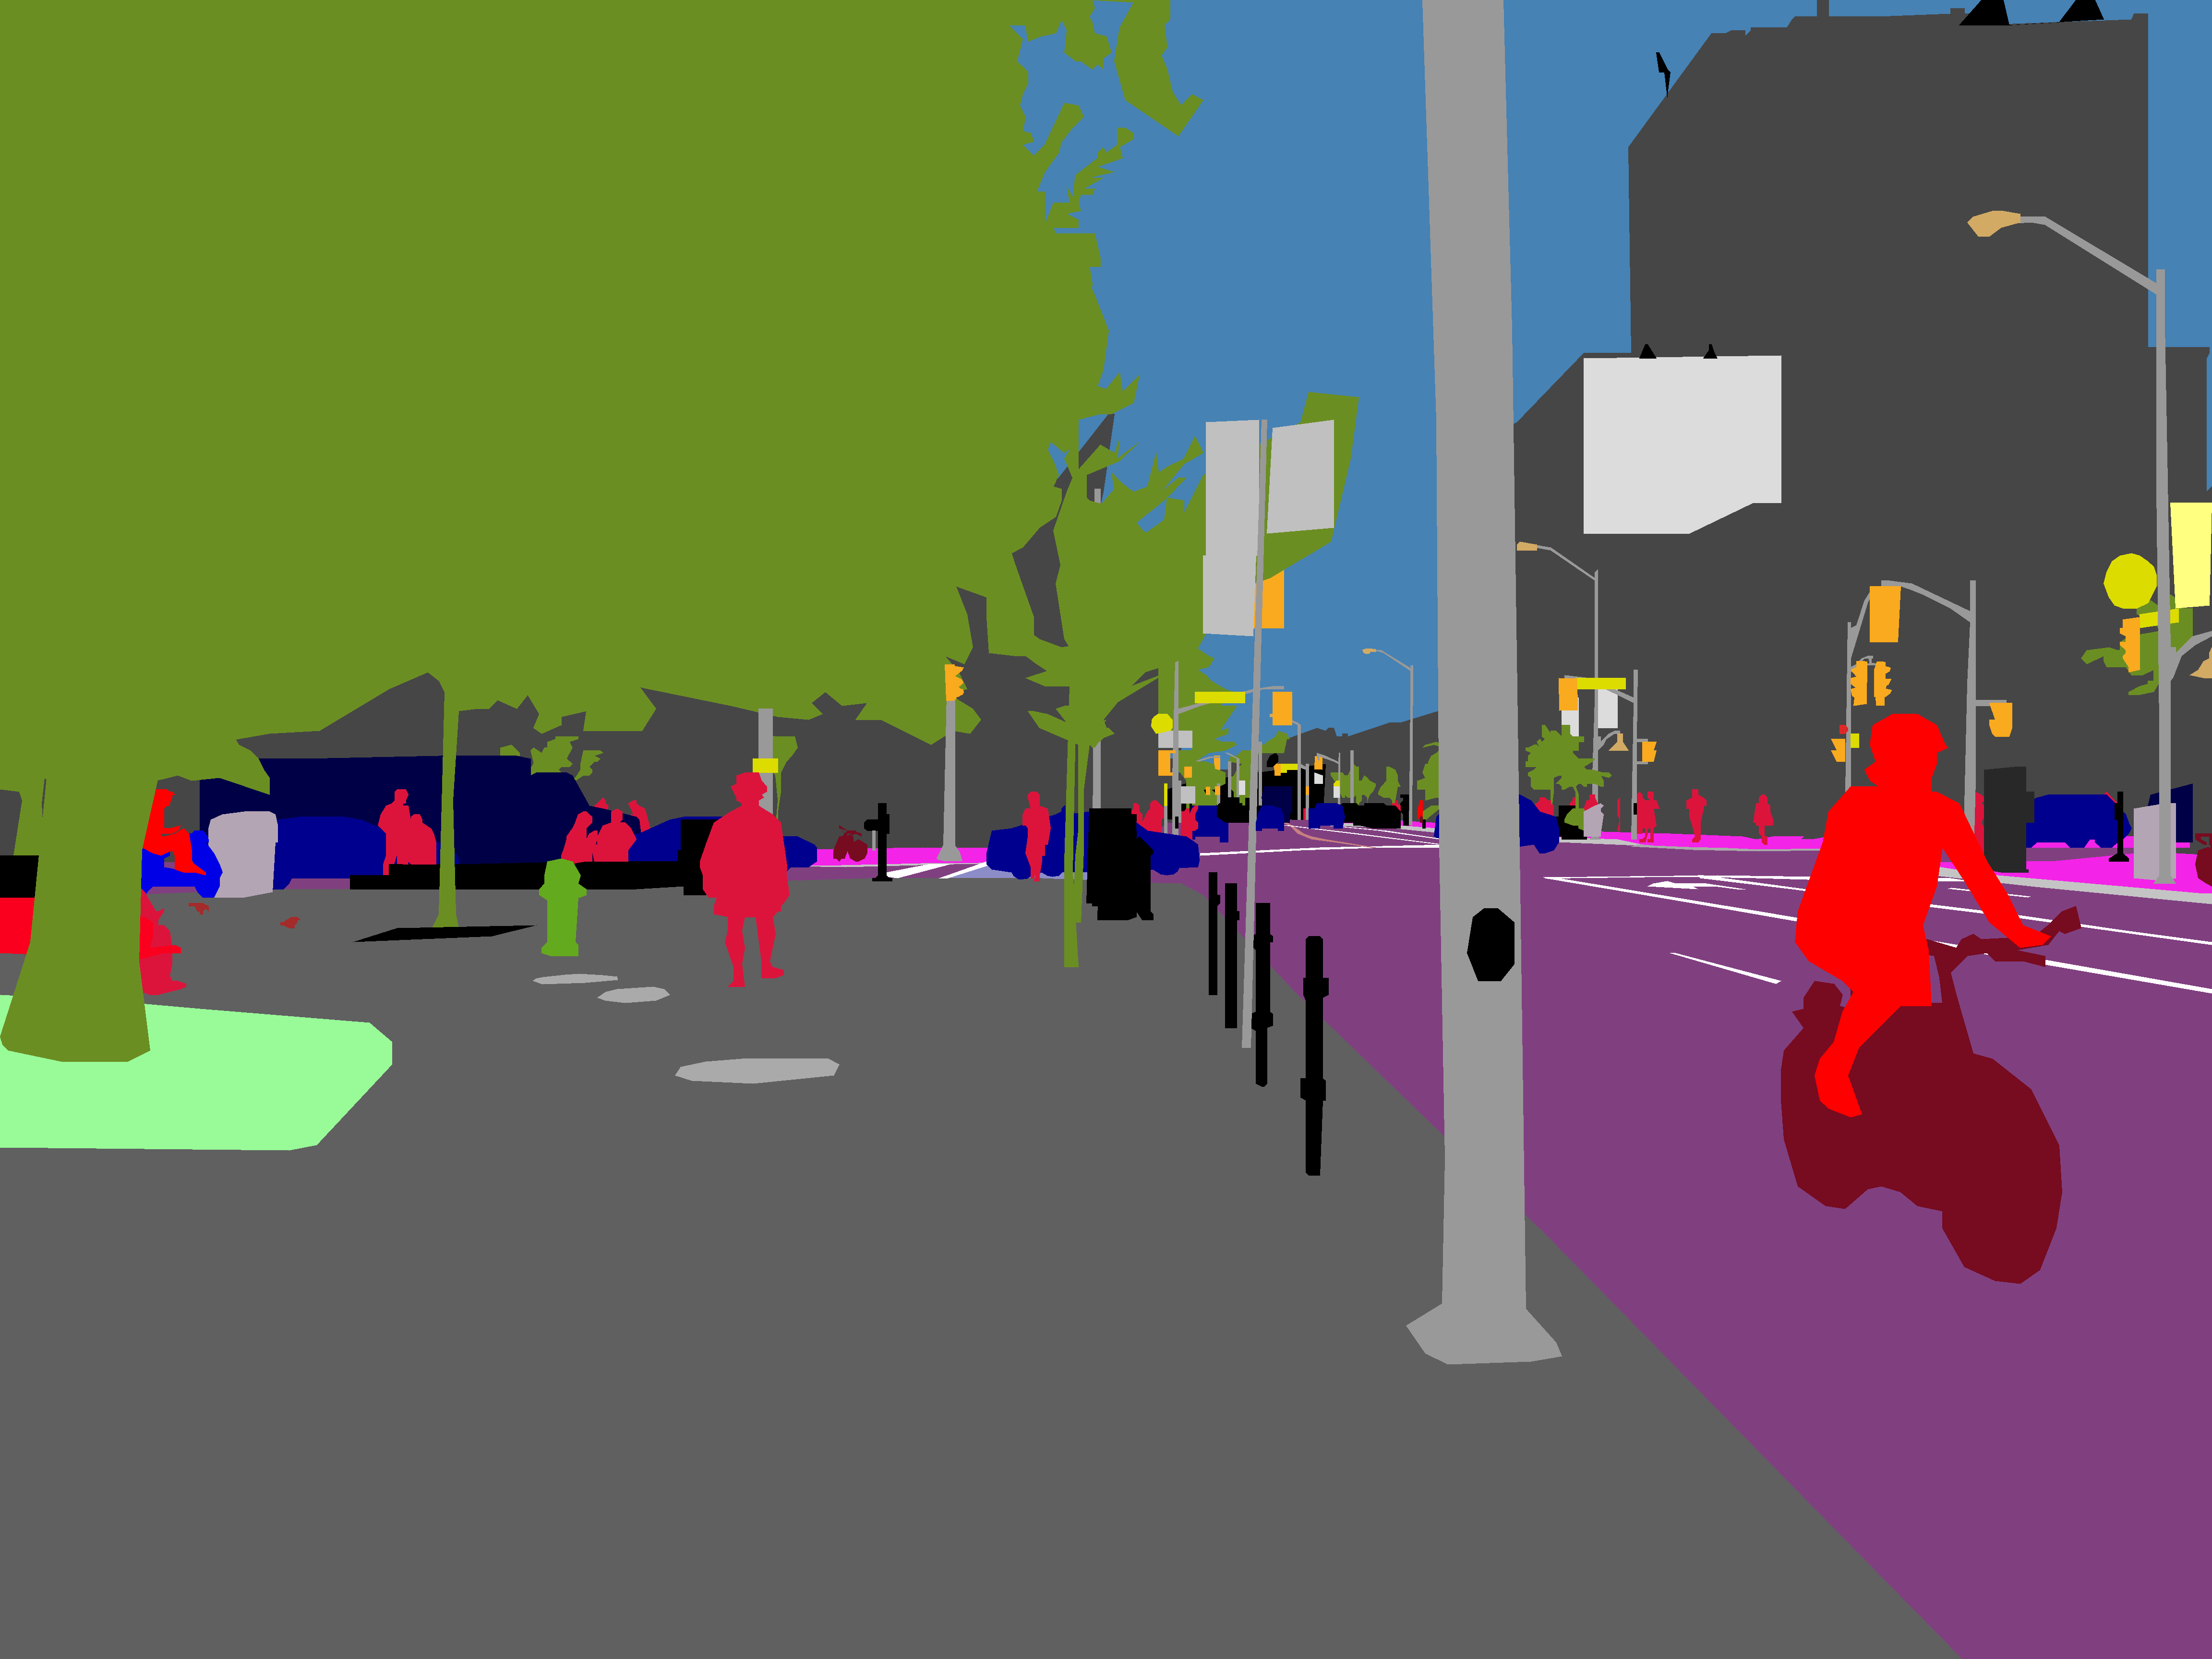
\includegraphics[height=1.5in]{recursos/imagens/semantic/s1.png}
        \caption{Segmentação semântica.}
        \label{semantic:fig:3.2}
    \end{subfigure}%

    Fonte: \cite{Neuhold2017_ICCV}.
\end{figure}

Portanto, neste capítulo, serão abordados tópicos relacionados às técnicas estado-da-arte no âmbito das arquiteturas de segmentação semântica, conforme detalhado na Seção \ref{semantic:arch}. Três variantes proeminentes serão discutidas nessa seção, buscando oferecer uma visão aprofundada dessas estratégias. Ademais, as métricas frequentemente utilizadas para avaliar a qualidade das segmentações semânticas serão minuciosamente detalhadas na Seção \ref{semantic:metrics}, fornecendo uma compreensão abrangente dos critérios de avaliação relevantes nesse tipo de abordagem.

\subsection{Arquiteturas}
\label{semantic:arch}
Quando abordamos as arquiteturas para os modelos de segmentação semântica, é evidente o crescente desenvolvimento de oportunidades para resolver a problemática de separar classes de objetos a nível de \textit{pixel}, como mencionado por \cite{Guo2018ANetworks}. No contexto das arquiteturas de segmentação semântica, existe uma divisão relevante relacionada ao nível de supervisão da rede, que inclui abordagens totalmente supervisionadas, fracamente supervisionadas e semi-supervisionadas, conforme detalhado por \cite{Hao2020ALearning}. No entanto, este trabalho se concentra exclusivamente nas arquiteturas consideradas estado-da-arte na parte totalmente supervisionada, pressupondo a disponibilidade de dados de treinamento rotulados, incluindo imagens originais juntamente com suas respectivas máscaras anotadas \citep{Hao2020ALearning}.

Para esmiuçar mais sobre essas arquiteturas, é importante ressaltar a diferença em relação às CNNs convencionais, que tendem a perder detalhes espaciais devido aos processos de \textit{pooling} e convoluções. As redes de segmentação semântica, ao contrário, são mais atentas a esses detalhes. Nesse contexto, a colaboração adequada entre esses dois tipos de características possui o potencial de aprimorar significativamente o desempenho da segmentação semântica, seguindo a estratégia denominada de \quotes{aprimoramento de recursos}, a qual será explorada adiante.

\subsubsection{\textit{Fully Convolutional Networks} (FCN)}
\label{semantic:FCN}
Quando aborda-se o tema das segmentações semânticas, vale dizer que arquiteturas e \textit{frameworks} foram desenvolvidos visando o avanço em termos de performance e capacidade. No entanto, o primeiro \textit{framework} a alcançar o status de estado-da-arte para esta tarefa de segmentação baseia-se na arquitetura  \textit{Fully Convolutional Networks} (FCN) \citep{Shelhamer2016}. Contrariamente às redes tradicionais que possuem camadas densas no final, a FCN é totalmente composta por camadas convolucionais, até mesmo na sua última camada \citep{Hesamian2019}.

Esta característica permite à FCN realizar uma análise \textit{pixelwise}, onde cada \textit{pixel} da imagem é subamostrado. Em seguida, através de processos de convolução e \textit{upsampling}, um mapa de segmentação semântica é construído. Este mapa de segmentação possui dimensões idênticas à imagem de entrada, o que permite a atribuição de uma classe semântica para cada \textit{pixel} \citep{Minaee2021, Zhang2018, Hesamian2019}.

A aplicação do FCN nos \textit{datasets} PASCAL VOC 2011 \citep{everingham2010pascal}, SIFT Flow \citep{Liu2011} e NYUDv2 \citep{Silberman:ECCV12}, resultou numa precisão de \textit{pixel} (PA) de 90,3\% e uma mIoU de 62,7\% no primeiro \textit{dataset} mencionado \citep{Ghosh2019}. O FCN, portanto, estabeleceu um novo patamar de referência quanto ao estado-da-arte em segmentação semântica \citep{Minaee2021} que antes era ocupado pelo modelo DeepLab \citep{Chen2017deeplab}.

A arquitetura da FCN é baseada nas arquiteturas das \textit{Convolutional Neural Networks} (CNNs) VGG-16 (explorada na Seção \ref{cnn:vgg}) e GoogLeNet \citep{Szegedy2015}. Esta adaptação permitiu que a FCN aceitasse entradas de tamanhos variáveis e produzisse saídas da mesma dimensão \citep{Minaee2021}, como pode ser visualizado na Figura \ref{semantic:fig:6}.

\begin{figure}[H]
    \centering
    \caption{Representação de exemplo em FCN.}
    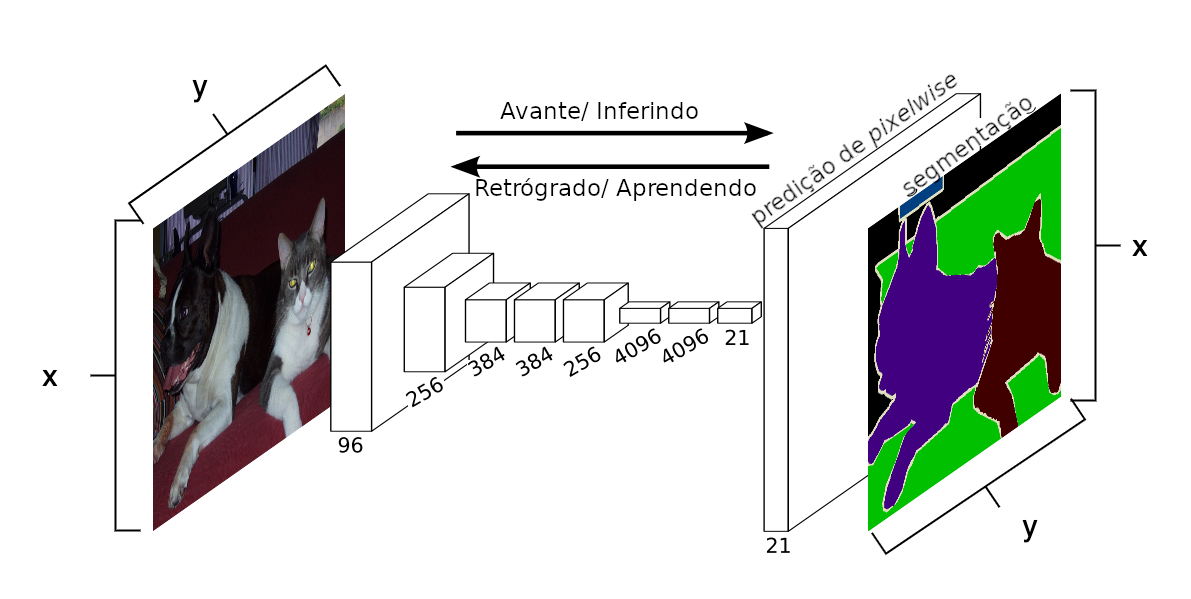
\includegraphics[width=1\linewidth]{recursos/imagens/semantic/fcn_example.png}
    \label{semantic:fig:6}

    Fonte: retirada e adaptado de \cite{Shelhamer2016}.
\end{figure}

Essas saídas, que são mapas de características do mesmo tamanho da imagem de entrada, podem ser utilizadas para várias aplicações. Por exemplo, em uma tarefa de detecção de objetos, cada \textit{pixel} da saída será classificado com a etiqueta do objeto à qual pertence, fornecendo portanto uma localização precisa dos objetos na imagem. Em uma aplicação de condução autônoma, a saída pode ser usada para identificar as zonas navegáveis ou obstáculos presentes na cena.

É relevante notar que a eficácia da FCN também está ligada ao seu mecanismo de subamostragem e amostragem ascendente, também conhecido como \textit{upsampling}. As camadas inferiores da rede capturam características locais, como bordas e texturas, enquanto as camadas superiores conseguem captar características de nível superior, como classes de objetos e suas relações espaciais \citep{Shelhamer2016}.

O desafio da subamostragem é que, enquanto ela contribui para a identificação de recursos em várias escalas e aumenta a eficiência computacional, também leva a uma perda de detalhes espaciais devido à redução da resolução da imagem. Para mitigar isso, a FCN implementa operações de \textit{upsampling}, que expandem a saída de baixa resolução para o tamanho original da imagem. Isso é realizado por meio de camadas de deconvolução ou interpolação, permitindo que a FCN produza uma segmentação densa em tempo de execução em uma única passagem para frente pela rede \citep{Shelhamer2016}.

Além disso, a FCN integra previsões de várias camadas em vários níveis de resolução, conhecido como saltos de conexões (ou em inglês, \textit{skip connections}), para refinar ainda mais a precisão da segmentação \citep{Minaee2021}. Com isso, a FCN consegue garantir que a segmentação semântica final esteja em conformidade tanto com as características de nível inferior quanto de alto nível, proporcionando resultados de segmentação precisos e detalhados.

Por fim, quanto às suas limitações, é informado que as configurações de FCN são ineficientes em trabalhos de segmentação 3D e para o uso em tempo real, visto que leva cerca de 100ms - em hardware não especificado pelo autor - para trabalhar com imagens de baixa resolução \citep{Minaee2021}, mas novas arquiteturas baseadas nesse modelo e na arquitetura ParseNet \citep{Liu2015} vêm evoluindo para suprir essas limitações.

\subsubsection{U-Net}
\label{semantic:unet}
No âmbito das arquiteturas voltadas para segmentação semântica, a evolução trouxe a U-Net \citep{Ronneberger2015U-net:Segmentation}, que se destacou após o período das FCNs. Introduzida em 2015, a U-Net rapidamente ganhou notoriedade, superando a popularidade das mencionadas FCNs \citep{Sultana2020EvolutionSurvey}.

As U-Nets operam com um caminho de contração (também conhecido como \textit{encoder}) que progressivamente reduz a resolução espacial dos dados e captura o contexto dos exemplos, seguido por um caminho de expansão simétrica (também conhecido como \textit{decoder}) que restaura a resolução original por meio de convoluções transpostas e realiza a segmentação. A estrutura se assemelha a um \quotes{U}, como retrata a Figura \ref{semantic:fig:unet}, o que levou à sugestão do nome da arquitetura. A conexão entre as camadas de \textit{encoder} e \textit{decoder}, conhecida como \quotes{\textit{skip connection}}, permite a preservação de informações de baixo nível e ajuda a mitigar problemas de perda de detalhes durante a redução da resolução \citep{Minaee2021, Minaee2021DeepClassification}. Por não conter camadas densas nas U-Nets, elas podem ser consideradas modelos baseados em FCNs \citep{Minaee2021}, sendo que a maior diferença entre essas arquiteturas está no uso de \quotes{\textit{skip connections}} entre as convoluções e \textit{upsamplings}, além da simetria das U-nets \citep{OZTURK2020ComparisonImageries}.

Vale citar que para a implementação de \quotes{up-samplings}, originalmente nas U-nets, foram utilizadas as convoluções transpostas com duas dimensões, que também são conhecidas como deconvoluções ou camada de deconvolução, realizando o processo contrário às camadas de \textit{pooling} \citep{Zeiler2014Visualizing2013}. Quando observa-se a parte técnica, essa camada é denominada \textit{Conv2DTranspose}, sendo que seu maior diferencial é que  ela amplia a resolução espacial dos dados, em oposição à redução feita pelas camadas de \textit{pooling}. No entanto, ao contrário das camadas de \textit{pooling}, a \textit{Conv2DTranspose} faz uso de uma janela de convolução para aumentar as dimensões dos dados. Essa camada é crucial para a U-Net, pois desempenha um papel fundamental na reconstrução das características espaciais, restaurando a resolução original e contribuindo para a precisão da segmentação, ao mesmo tempo em que mantém as conexões entre as características de nível mais baixo e mais alto, garantindo a riqueza dos detalhes na segmentação final.

\begin{figure}[H]
    \centering
    \caption{Arquitetura U-Net.}
    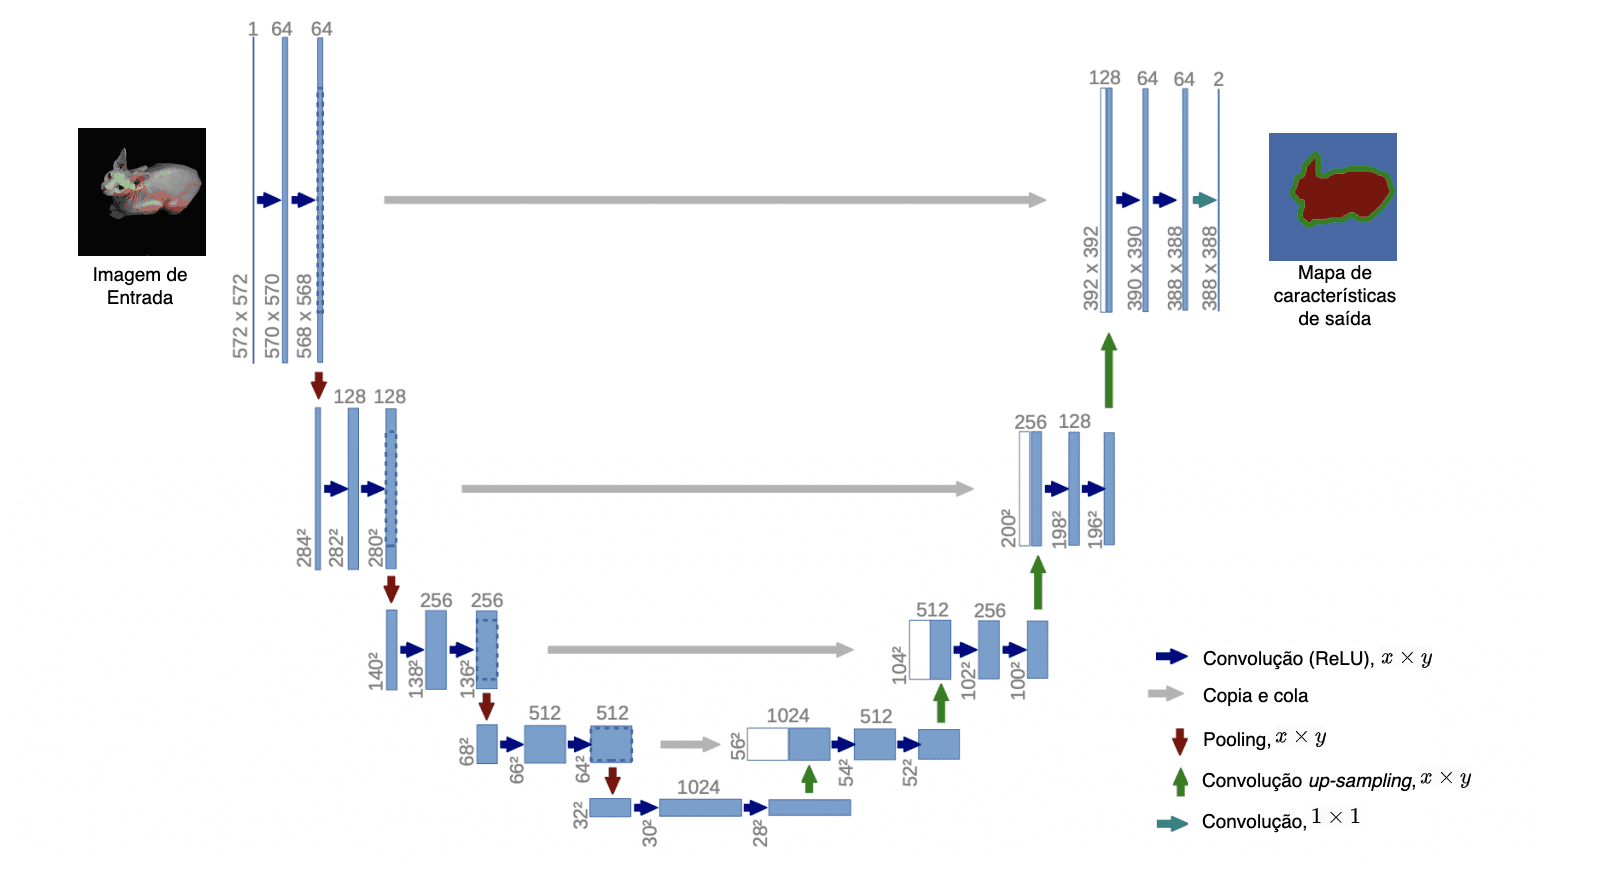
\includegraphics[width=1\linewidth]{recursos/imagens/semantic/unet-arch.png}
    \label{semantic:fig:unet}

    Fonte: retirada e adaptado de \cite{Ronneberger2015U-net:Segmentation}.
\end{figure}

As vantagens inerentes a essa arquitetura incluem uma capacidade robusta para lidar com imagens de tamanhos variados, permitindo a aplicação eficiente em diversos contextos, como na análise de imagens médicas \citep{Ronneberger2015U-net:Segmentation}. Além disso, as U-Nets têm a habilidade de aprender representações altamente significativas em diferentes níveis de abstração, o que as torna eficazes na captura de detalhes importantes em uma imagem \citep{Alom2019RecurrentSegmentation}. Também é importante destacar que essas redes têm a capacidade de reduzir a tendência de gerar segmentações excessivamente granulares, fornecendo segmentações mais suaves e coerentes \citep{Du2020MedicalReview}. No entanto, é fundamental reconhecer que, como qualquer abordagem, as U-Nets também possuem desvantagens. Em particular, essas redes frequentemente possuem um grande número de parâmetros, o que pode aumentar os requisitos computacionais e tornar o treinamento mais demorado, dependendo do tamanho do conjunto de dados e da complexidade da tarefa \citep{Ronneberger2015U-net:Segmentation}. Além disso, pela grande quantidade de convoluções, muitas vezes a informação espacial é perdida, segundo \cite{Zhang2023LcmUNet:Segmentation}.

Voltando ao contexto mais amplo, onde a segmentação semântica tem como objetivo atribuir rótulos de classe a cada \textit{pixel} em uma imagem, a arquitetura da U-Net se mostra relevante e eficaz, sendo exemplificado pelos resultados obtidos desde seu desenvolvimento com \cite{Ronneberger2015U-net:Segmentation}. No entanto, questões que exploram a preservação da espacialidade da imagem durante a segmentação nesse tipo de estrutura ainda são pouco explorados, principalmente quando a proposta está em variações das tradicionais camadas de \textit{pooling} que são os atuais estado-da-arte.

\subsubsection{U-Net-\textit{Like}}
\label{semantic:unetlike}
Após o surgimento e o êxito alcançado pelas U-Nets, surgiram variações dessas redes, frequentemente denominadas de U-Net-\textit{Like}, inspiradas pela estrutura original proposta por \cite{Ronneberger2015U-net:Segmentation} e amplamente documentada em \citep{Kugelman2022ASegmentation}.

Essas redes mantêm a arquitetura de contração e expansão da U-Net original, mas apresentam características distintas. Uma das diferenças significativas é a adição de \textit{skip connections} com a inclusão de uma camada extra, a incorporação de técnicas como \textit{Batch Normalization} proposta por \cite{Ioffe2015BatchShift} e a função de ativação ReLU, discutida na Seção \ref{deep:relu}, nas camadas de contração. Essas alterações têm como objetivo manter as médias e variâncias das entradas constantes, acelerando o aprendizado e aumentando a estabilidade durante a fase de treinamento \citep{Pfister2019AutomatedNetworks}.

Outra modificação presente nas U-Net-\textit{Like} diz respeito à forma como as convoluções são aplicadas. Enquanto \cite{Ronneberger2015U-net:Segmentation} não aplicava preenchimento (\textit{padding}) devido ao processo de divisão de imagens maiores em blocos menores durante o processamento, a abordagem das U-Net-\textit{Like} introduz \textit{pixels} adicionais ao redor das bordas da imagem. Esse procedimento permite que as convoluções utilizem \textit{pixels} vizinhos, aprimorando a eficiência e a qualidade da segmentação \citep{Pfister2019AutomatedNetworks}.

Dentre os últimos detalhes, vale dizer que diferente do método de \textit{up-sampling} com as convoluções transpostas em duas dimensões, esse método utiliza de um método chamado originalmente de \textit{Upsampling2D}, o qual emprega uma abordagem diferente para aumentar a resolução espacial dos dados. Enquanto as convoluções transpostas realizam a ampliação por meio do aprendizado de pesos, o método \textit{Upsampling2D} opera replicando os valores existentes nos mapas de características, efetivamente duplicando-os e, assim, aumentando a resolução espacial. Além disso, sua maior mudança em relação às convoluções transpostas em duas dimensões se dá pela ausência de parâmetros treináveis, resultando em uma operação mais simples e menos custosa computacionalmente.

Finalmente, vale dizer que no uso das U-Net-\textit{Like} é possível visualizar uma diminuição dos parâmetros de treinamento da rede \citep{Pfister2019AutomatedNetworks}, contribuindo para uma arquitetura mais enxuta e eficiente. Além disso, o uso do \textit{Upsampling2D} nas U-Net-\textit{Like} implica não só em uma redução de parâmetros, mas também em um processo de treinamento mais rápido e menos complexo, uma vez que essa abordagem não requer parâmetros treináveis adicionais, proporcionando uma operação computacionalmente mais leve e uma convergência mais ágil durante o treinamento.

\subsection{Métricas}
\label{semantic:metrics}
Considerando que o objetivo principal das segmentações semânticas está relacionado à atribuição de classes para cada um dos \textit{pixels} presentes na imagem \citep{Csurka2013}, é fundamental o uso de métricas para avaliar o desempenho positivo ou negativo dos modelos.

Nesta seção, serão discutidas métricas comuns para avaliação de segmentações semânticas: métricas baseadas em região, como a precisão de \textit{pixel} (Seção \ref{semantic:pa}), a interseção sobre a união (Seção \ref{semantic:IoU}) e sua variação, a média da interseção sobre a união (Seção \ref{semantic:miou}), e por fim, o escore F1 (ou F1 \textit{score}) (Seção \ref{semantic:f1}).


\subsubsection{\textit{Pixel Accuracy}}
\label{semantic:pa}
A métrica de \textit{pixel accuracy} (PA) é uma das métricas mais simples utilizadas no contexto de segmentação semântica, em que, na prática, se resume na razão entre o número de \textit{pixels} classificados corretamente em relação ao total de \textit{pixels} na imagem \citep{Minaee2021}. Sendo assim, é possível expressar a sua fórmula pela Equação \ref{semantic:eq:1} \citep{Minaee2021}:

\begin{equation}
    \label{semantic:eq:1}
    PA = \frac{\sum_{i=0}^{K} p_{ij}}{\sum_{i=0}^{K} \sum_{j=0}^{K} p_{ij}},
\end{equation}
sendo $K$ o número de classes presentes na imagem, independente se para um plano de fundo ou para primeiro plano, e $p_{ij}$ é o número de \textit{pixels} preditos como $i$ pertencentes à classe $j$.

Todavia, é relevante citar que essa métrica indicando apenas precisão dos \textit{pixels}, como o nome sugere, não é adequada para situações que há um desequilíbrio de classes, situação em que determinadas classes dominam a cena e que se faz presente no mundo real.


\subsubsection{\textit{Intersection over Union} (IoU)}
\label{semantic:IoU}
Já a métrica de intersecção entre a união, do inglês \textit{Intersection over Union} (IoU) ou Jaccard Index, é uma métrica que não passa por problemas de desbalanceamento de classes, além de ser considerada uma das métricas mais comuns para esse tipo de atividade \citep{Minaee2021}.

Sua representação pode ser visualizada a partir da Figura \ref{semantic:fig:1}, além de que pela Equação \ref{semantic:eq:2} é possível entender que o resultado de $IoU$ se dá pela razão entre a intersecção das áreas da segmentação predita (A) e \textit{ground truth} (B), e a união entre a segmentação predita e o \textit{ground truth}, ou seja,

\begin{equation}
    \label{semantic:eq:2}
    IoU = J(A,B) = \frac{|A \cap B|}{|A \cup B|}.
\end{equation}

\begin{figure}[H]
    \centering
    \caption{Representação de IoU.}
    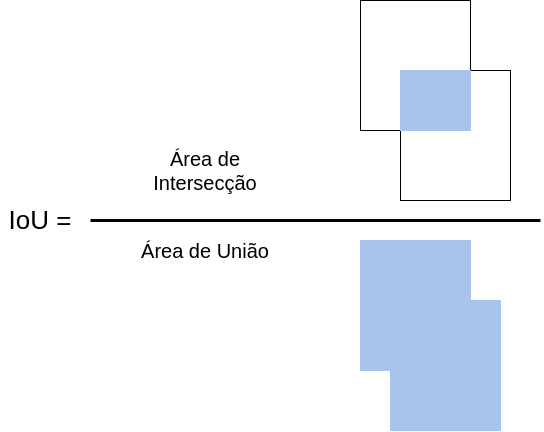
\includegraphics[height=2.3in]{recursos/imagens/semantic/IoU.png}
    \label{semantic:fig:1}

    Fonte: do próprio autor.
\end{figure}

\subsubsection{\textit{Mean Intersection Over Union} (MIoU)}
\label{semantic:miou}
Após a introdução da métrica IoU, outras variações ganharam destaque, destacando-se o \textit{Mean Intersection-over-Union} (mIoU), que calcula a média dos valores de IoU para todas as classes presentes na cena, fornecendo um valor escalar como resultado para a segmentação como um todo \citep{Minaee2021}. Esta métrica tem sido empregada em estudos relevantes, como exemplificado por \cite{Mohan2020}.

É relevante ressaltar que métricas como mIoU e \textit{Mean Average Precision} (mAP), em relação à métrica \textit{Average Precision} - também comentadas por \cite{Padilla2021} - possuem maior relevância na análise de problemas com múltiplas classes ou objetos, permitindo medir a capacidade de generalização do modelo em questão.

A Equação \ref{semantic:eq:miou} pode ser utilizada para ilustrar o funcionamento do $mIoU$, onde $N$ é o número de regiões no conjunto de dados e as demais variáveis são baseadas na Equação \ref{semantic:eq:2}:

\begin{equation}
    \label{semantic:eq:miou}
    mIoU = \frac{\sum_{i=1}^N IoU(A_i, B_i)}{N}.
\end{equation}

\subsubsection{F1-\textit{Score}}
\label{semantic:f1}
Para a definição da métrica F1-\textit{score}, que é comum na esfera de segmentação de imagens, é necessário ter ciência de antemão que ela é composta pelo uso de outras duas métricas, sendo elas: 1) precisão, que é a divisão de verdadeiros positivos ($VP$) pela soma de verdadeiros positivos ($VP$) e falsos positivos ($FP$); 2) revocação, que é a divisão de verdadeiros positivos ($VP$) pela soma de verdadeiros positivos ($VP$) e falsos negativos ($FN$), como mostrados nas Equações \ref{semantic:eq:3} e \ref{semantic:eq:4}, respectivamente,

\begin{equation}
    \label{semantic:eq:3}
    \text{Precisão} = \frac{VP}{VP + FP}
\end{equation}
e
\begin{equation}
    \label{semantic:eq:4}
    \text{Revocação} = \frac{VP}{VP + FN}.
\end{equation}

Assim, para a definição de F1-\textit{score} é utilizada a média harmônica entre a precisão e revocação \citep{Minaee2021}, a qual pode ser expressa pela Equação \ref{semantic:eq:5}:

\begin{equation}
    \label{semantic:eq:5}
    F1-score = \frac{2 \cdot \text{Precisão} \cdot \text{Revocação}}{\text{Precisão} + \text{Revocação}}.
\end{equation}

Por fim, vale comentar que para situações em que tem-se uma segmentação binária. O valor de F1-\textit{score} é semelhante ao valor do coeficiente Dice, o qual normalmente é utilizado para situações médicas \citep{Minaee2021} e utiliza conceitos de intersecção assim como a métrica de IoU (Seção \ref{semantic:IoU}), visto que quando não está assimilado a situações binárias, pode ser representado pela Equação \ref{semantic:eq:6} ou pela Figura \ref{semantic:fig:2}:

\begin{equation}
    \label{semantic:eq:6}
    Dice = \frac{2|A \cap B|}{|A| + |B|}.
\end{equation}

\begin{figure}[H]
    \centering
    \caption{Representação do coeficiente Dice.}
    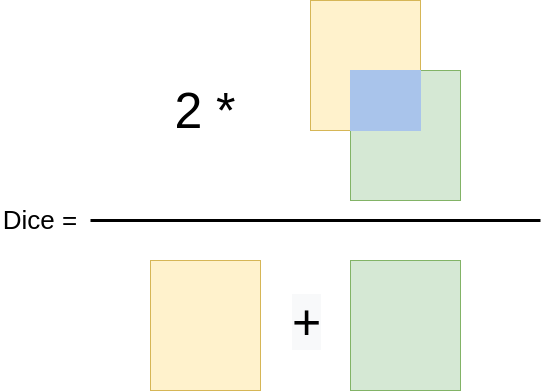
\includegraphics[height=2.3in]{recursos/imagens/semantic/dice.png}
    \label{semantic:fig:2}

    Fonte: do próprio autor.
\end{figure}

\subsection{Considerações Finais do Capítulo}
\label{semantic:conclusion}
Em conclusão sobre as segmentações semânticas, é notável o avanço significativo em comparação com tarefas de detecção de objetos, como destacado em \cite{Vaillant1994}. Esses novos modelos de segmentação permitem o trabalho com um volume maior de dados em cenas complexas, como abordado neste capítulo.

No entanto, é importante ressaltar que essas redes enfrentam dificuldades quando o problema requer a separação de objetos da mesma classe, mas distintos e sobrepostos, resultando na ausência de uma segmentação individualizada \citep{Kirillov2019a}. Isso fica evidente na Figura \ref{semantic:fig:4}, onde pessoas próximas estão conectadas, ou em situações que exigem uma segmentação detalhada da cena \citep{Ghosh2019}.

\begin{figure}[H]
   \caption{Exemplo de segmentação semântica com instâncias unificadas.}
   \centering
   \label{semantic:fig:4}
    \begin{subfigure}[t]{0.8\textwidth}
        \centering
        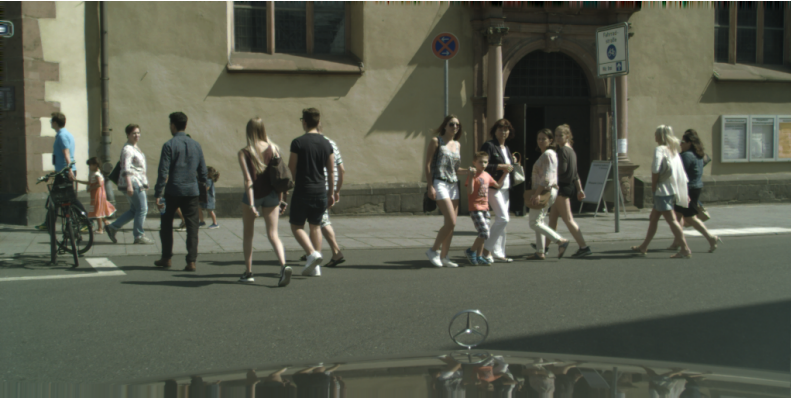
\includegraphics[width=1\linewidth]{recursos/imagens/semantic/sema_ori.png}
        \caption{Imagem original.}
        \label{semantic:fig:4.1}
    \end{subfigure}%
    ~ 

    \begin{subfigure}[t]{0.8\textwidth}
        \centering
        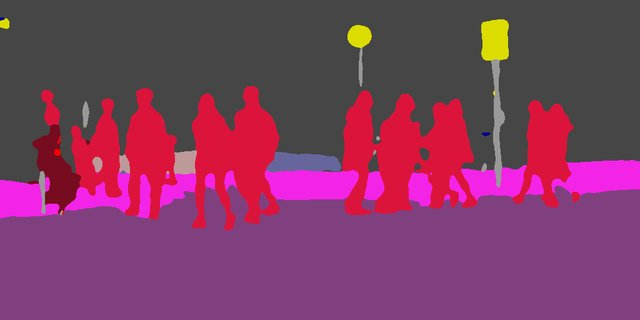
\includegraphics[width=1\linewidth]{recursos/imagens/semantic/sema_unified.png}
        \caption{Segmentação com instâncias unificadas.}
        \label{semantic:fig:4.2}
    \end{subfigure}%

    Fonte: \cite{Fischer2017}.
\end{figure}

É válido mencionar a emergência de abordagens estado da arte e arquiteturas baseadas em \textit{transformers}, que têm demonstrado excelente desempenho em uma variedade de tarefas de visão computacional, incluindo segmentação semântica. No entanto, considerando que o foco deste trabalho estavam mais focados nas questões de \textit{pooling} e nas arquiteturas clássicas de aprendizado profundo, essas abordagens mais novas, embora notáveis, estiveram fora do escopo da discussão atual.

Por fim, é importante ressaltar que os modelos de segmentação semântica podem não ser ideais para sistemas que requerem segmentações em tempo real, especialmente ao operar com câmeras que capturam menos de 25 quadros por segundo. Isso se deve ao seu custo computacional elevado, o qual pode dificultar a obtenção de resultados em tempo hábil para aplicações em tempo real. Essa limitação foi identificada e discutida por \cite{Minaee2021}. Além disso, é fundamental considerar as questões relacionadas ao desempenho das métricas de avaliação do modelo quando se busca preencher essa lacuna de tempo, visando compreender como os modelos se comportam em condições de processamento em tempo real. Essa análise é crucial para determinar a viabilidade e eficácia desses modelos em aplicações práticas que demandam segmentação em tempo real \citep{badrinarayanan2017segnet}.